\documentclass{report}
\usepackage{float}
\usepackage{amsmath, amssymb}
\usepackage{graphicx}
\newcommand{\overbar}[1]{\mkern 1.5mu\overline{\mkern-1.5mu#1\mkern-1.5mu}\mkern 1.5mu}
\newcommand{\subsubsubsection}[1]{\paragraph{#1}\mbox{}\\}
\title{%
    Metodi matematici per l'informatica \\    
    \large Corso del professore Carlucci
    \large https://sites.google.com/uniroma1.it/mmi2223/home
}
\author{Lugini Andrea}
\begin{document}
\maketitle
\tableofcontents
\newpage 
\section{Tecniche di conteggio: Matematica combinatoria}
    La matematica combinatoria è la branca della matematica che si occupa dei problemi
    di conteggio. \\
    Ad esempio il problema del numero di targe automobilistiche disponibili al mondo
    ricade in questo ambito. \\
    \subsection{Principio Moltiplicativo}
        Se scelgo un primo oggetto fra $m_1$, un secondo oggetto tra $m_2$, ..., un 
        t-esimo oggetto fra $m_t$ oggetti ho $m_1 \cdot m_2 \cdot ... \cdot m_t$ soluzioni.
    \subsection{Disposizioni}
    Le disposizioni sono sequenze nelle quali l'ordine conta.
        \subsubsection{Disposizioni con ripetizione di ordine k di n oggetti}
            $$D_{n,k}^{'} = n^k$$
        \subsubsection{Disposizioni semplici di ordine k di n oggetti}
            $$C.E. = 1 \leq k \leq n$$
            $$D_{n,k} = \frac{n!}{(n - k)!}$$
            Nel caso $k = n$, parliamo di permutazioni e abbiamo: $P_{n} = n!$.
        \subsubsection{Permutazioni con ripetizioni}
            Presi n elementi, che si \textbf{ripetono rispettivamente} $k_1, ..., k_n$ volte, le
            possibili permutazioni sono: 
            $$P_{n}^{k_1, ..., k_n} = \frac{n!}{k_1! \cdot ... \cdot k_n!}$$
        \subsubsection{Permutazioni di n oggetti con q vincoli}
            $$\frac{P_{n}}{q!}$$
    \subsection{Combinazioni}
    Le combinazioni sono sequenze nel quale l'ordine non conta
        \subsubsection{Combinazioni semplici}
            $$C_{n,k} = \frac{D_{n,k}}{P_k} = \binom{n}{k} = \frac{n!}{k! \cdot (n-k)!}$$
        \subsubsection{Combinazioni con ripetizione}
            Risolvono il problema della \textbf{scritture additive} e della distribuzione
            di k oggetti identici tra n insiemi
            $$C_{n,k}^{'} = \binom{n + k - 1}{k-1}$$
    \subsection{Proprietà del coefficiente binomiale}
        $$\binom{n}{k} = \binom{n}{n-k}$$
        Dimostrazione per \textbf{doppio conteggio}: con $\binom{n}{k}$ scelgo k oggetti su n,
        lasciando fuori $n-k$ oggetti. E' quindi equivalente scegliere gli
        $n-k$ oggetti da lasciare fuori, ovvero $\binom{n}{n-k}$ \\
        $$\binom{n}{k} = \binom{n-1}{k-1} + \binom{n-1}{k}$$
        Dimostrazione per \textbf{partizioni}: dato un insieme N di cardinalità n
        nel quale vogliamo scegliere k oggetti sappiamo che il numero di possibili
        soluzioni sono $\binom{n}{k}$.
        Se vogliamo inserire vincoli specifici di scelta, ovvero scegliere k oggetti,
        tra i quali un oggetto x, nell'insieme n, la totalità dei 
        sottoinsiemi che contengono x è data dalla scelta fissa $x \cdot$ le \textbf{combinazioni}
        dei restanti $k-1$ oggetti fra $n-1$ elementi, ovvero $\binom{n-1}{k-1}$.
        Se invece vogliamo vedere il problema al contrario, ovvero scegliere k oggetti,
        tra i quali \textbf{non vogliamo x}, dobbiamo scegliere k oggetti su $n-1$
        elementi, quindi $\binom{n-1}{k}$. Per partizione abbiamo quindi che la totalità
        delle scelte è data dall'unione delle scelte che includono x e quelle che non includono
        x, insiemi \textbf{disgiunti}, è quindi è dimostrata la formula. \\
        $$\binom{n}{m} \cdot \binom{m}{k} = \binom{n}{k} \cdot \binom{n-k}{m-k}$$
        Dimostrazione per \textbf{doppio conteggio}: il primo termine a sinistra
        sveglie m oggetti su n elementi, e il secondo mi fa scegliere
        k oggetti fra gli m scelti prima. A destra scegliamo k oggetti su n,
        e poi scegliamo $m-k$ oggetti sui restanti $n-k$. \\
        Esempio: \\
            Vogliamo fare una squadra di calcio con 3 portieri e 10 giocatori di movimento, 
            scegliendo fra 30 bambini. \\
            A sinistra scegliamo prima i 13 bambini che giocheranno a calcio e poi 
            sceglieremo i 3 fra questi 13 che faranno i portieri. \\
            A destra invece scegliamo prima i 3 portieri fra i 30 bambini, e poi
            sceglieremo i 10 giocatori di movimento fra i restanti 30 tolti i 3 portieri bambini.
    \subsection{Principio additivo}
        Il principio additivo ci permette di risolvere un problema di conteggio
        \textbf{sommando le numerosità} di n sottoinsiemi, detti \textbf{partizioni} dell'insieme da contare,
        se e solo se i sottoinsieme suddividono la collezione in gruppi \textbf{esclusivi ed esaustivi}.
        E' esprimibile come:
        $$ \forall i \in \{1, ..., n\}: A_i \subseteq A \; \wedge $$
        $$ \forall i,j \in \{1, ..., n\} \textrm{ con } i \neq j: A_i \cap A_j = \emptyset \; \wedge $$
        $$ \forall a \in A: \exists i \in \{1, ..., n\} \textrm{ t.c. } a \in A_i \ $$
        $$ \Longrightarrow \#A = \Sigma_{i=1}^{n} \#A_i $$
        \subsubsection{Metodo inverso}
            Il principio additivo ci permette di dimostrare il metodo inverso. \\
            Infatti, preso un sottoinsieme A di T ed il suo complementare $\overbar{A}$ in T, definito come
            $\forall x \in T \textrm{ t.c. } x \notin A$, per i quali valgono quindi le proprietà
            $A \cup \overbar{A} = T$ e $A \cap \overbar{A} = \emptyset$, è dimostrato quindi 
            il principio additivo, che ci permette di calcolare $\#T$ come $\#A + \#\overbar{A}$, che implica
            $$\#A = \#T - \#\overbar{A}$$.
    \subsection{Insieme potenza}
        $$P(A) = \{S | S \subseteq A\}$$
        $$\#P(A) = \Sigma_{k=0}^{\#A}\binom{\#A}{k} = 2\cdot\Sigma_{k=0}^{\#A/2}\binom{\#A}{k}$$
        Dimostriamo ora per \textbf{buona traduzione} che $\#P(A) = 2^{\#A}$: \\
        prendiamo due linguaggi, $L_1$, che rappresenta tutti $S \in P(A)$, ed
        $L_2$, che rappresenta tutte le possibili \textbf{stringhe binarie} di 
        lunghezza $ = \#A$; se costruiamo queste stringhe ponendo in posizione
        $i$ 1 se $e \in S$ e 0 in caso contrario, possiamo notare che, poichè
        ogni $S \in P(A)$ è distinto, anche le corrispondenti stringhe saranno distinte. \\
        Quindi, $\#P(A) = \#\textrm{stringhe binarie con l} = \#A$, ed è banale contare 
        quante stringhe sono presenti in $L_2$: 2 possibili valori, 0 ed 1, per $\#A$
        posizioni, ovvero $2^{\#A}$, esattamente quello che volevamo dimostrare. \\
        Possiamo inoltre notare che $\binom{n}{k} = \#\textrm{stringhe binarie con l} = \#A
        \textrm{ con esattamente k "1"}$.
    \subsection{PIE: Principio di inclusione ed esclusione}
        L'insieme $Q$ dato da tutti gli elementi distinti degli insiemi $A$ e $B$
        è esprimibile come $(A \cup B) \cap \overline{A \cap B}$. \\
        Quindi:
        $$\#\left(A \cup B\right) = \#A + \#B - \#\left(A \cap B\right)$$
        Più genericamente,
        $$\#\left(A \cup B \cup ... \cup Z\right) = $$
        $$\#A + \#B + ... + \#Z$$
        $$ - \#\left(A \cap B\right) - \#\left(A \cap Z\right) - \left(B \cap Z\right) - ... $$
        $$ + \#\left(A \cap B \cap Z\right) + ... $$
    \subsection{Metodo di riduzione}
        Il metodo di riduzione consiste nel trasformare un problema in un problema
        più semplice.
\newpage 
\section{Funzioni}
    $$ f: I \longrightarrow O $$
    \subsection{Definizione}
        Una funzione è una legge che, preso l'insieme di partenza $I$ detto dominio, e 
        l'insieme di arrivo $O$ detto codominio, $\exists!y \textrm{ t.c. } y = f\left(x\right)$.
    \subsection{Immagine e pre-immagine}
        $y \in O \textrm{ t.c. } y = f\left(x \in I\right)$ è detta immagine di $x$ via $f$. \\
        $x \in I \textrm{ t.c. } y \in O = f\left(x\right)$ è detta pre-immagine di $y$ via $f$
    \subsection{Definizione insiemistica}
        Presi $I$ e $O$, $f: I \longrightarrow O \subseteq (I \cdot O) \textrm { t.c. }
        \forall x \in I \exists! y \in O \textrm{ t.c. } \left(x,y\right) \in f$ \\
    \subsection{Funzioni a più argomenti}
        Una funzione a più argomenti può essere vista come una funzione che ha 
        $$I = I_1 \cdot I_2 \cdot ...$$
        ed e quindi formata da \textbf{n-tuple ordinate}. \\
        La notazione usata in questo caso è:
        $$f: I^n \longrightarrow O$$
    \subsection{Iniettività, Suriettività e Biettività}
        Iniettiva: $\forall x,y \textrm{ t.c. } x \neq y \Longrightarrow f\left(x\right) \neq f\left(y\right)$ \\
        Suriettiva: $\forall y \in O \exists x \in I \textrm{ t.c. } y = f\left(x\right)$ \\
        Biettiva: Iniettiva $\wedge$ suriettiva.
        \subsubsection{Proprietà dell'iniettiva}
            $$f: X \longrightarrow Y, f \textrm{ iniettiva } \Longrightarrow \exists g: Y \longrightarrow X \textrm{ t.c. } \left(g \circ f\right)\left(x\right) = x$$
            La dimostrazione è alquanto semplice. \\
            Se $y \in f\left(X\right) \Longrightarrow \exists! x \in X \textrm{ t.c. } f\left(x\right) = y$ in quanto $f$ iniettiva. \\
            Se invece $y \notin f\left(X\right)$ allora non ci interessa il comportamento di $g\left(y\right)$.
        \subsubsection{Implicazione dell'esistenza di $g$}
            $$\exists g: Y \longrightarrow X \left(g \circ f\right)\left(x\right) = x \Longrightarrow f \textrm{ iniettiva }$$.
            Procediamo per assurdo, ipotizzando che f non sia iniettiva. \\
            Allora esisterebbero due valori $x_0, x_1 \in X, x_0 \neq x_1 \textrm{ t.c. } f\left(x_0\right) = f\left(x_1\right)$.
            Sappiamo inoltre che $\left(g\circ f\right)\left(x_0\right) = x_0$ e $\left(g \circ f\right)\left(x_1\right) = x_1$.
            In quanto $g$ l'inversa di $f$ e $f\left(x_0\right) = f\left(x_1\right)$ allora 
            $$\left(g\circ f\right)\left(x_0\right) = \left(g \circ f\right)\left(x_1\right) \Longrightarrow x_0 = x_1$$
            Situazione impossibile per ipotesi.
            \subsubsubsection{Corollario}
                $$f \textrm{ iniettiva } \Longleftrightarrow \exists g \textrm{ t.c. } \left(g \circ f\right)\left(x\right) = x$$
        \subsubsection{Proprietà della suriettività}
            $$f: X \longrightarrow Y, f \textrm{ suriettiva } \Longrightarrow \exists g: Y \longrightarrow X \textrm{ t.c. } \left(f \circ g\right)\left(y\right) = y$$
            Anche qui la dimostrazione è alquanto banale. \\
            Infatti, prendendo un qualunque $y \in Y$ basta prendere $x \textrm{ t.c. } f\left(x\right) = y$, la cui esistenza è garantita dalla suriettività di $f$. \\
            Potrebbero esserci diverse $x \in X$ che soddisfano questa relazione, ma non è importanti quali scegliamo.
        \subsubsection{Implicazione dell'esistenza di $g$}
            $$\exists g: Y \longrightarrow X \textrm{ t.c. } \left(f \circ g\right)\left(y\right) = y \Longrightarrow f \textrm{ suriettiva }$$
            Procediamo per assurdo, ipotizzando che f non sia suriettiva.
            Questo implica che $\exists y \in Y \textrm{ t.c. } \nexists x \in X \textrm{ t.c. } y = f\left(x\right)$.
            Però per ipotesi $f\left(g\left(y\right)\right) = y \Longrightarrow \exists x \in X \textrm{ t.c. } y = f\left(x\right)$, 
            in contraddizione con quanto definito prima.
            \subsubsubsection{Corollario}
                $$f \textrm{ suriettiva } \Longleftrightarrow \exists g \textrm{ t.c. } \left(f \circ g\right)\left(x\right) = x$$
    \subsection{Proprietà insiemistiche delle funzioni}
        Presi $A,B \subseteq I$:
        $$f \textrm{ iniettiva } \Longrightarrow f\left(A \cap B\right) = f\left(A\right) \cap f\left(B\right)$$
        $$f\left(A \cup B\right) = f\left(A\right) \cup f\left(B\right)$$
    \subsection{Composizione di funzioni}
        Prese $f: X \longrightarrow Y$ e $g: Y \longrightarrow Z, \, g \circ f = 
        h: X \longrightarrow Z \textbf{ definita come } h\left(x\right) = g\left(f\left(x\right)\right)$ \\
        La composizione di funzione \textbf{non è commutativa} ma è \textbf{associativa} \\
        \subsection{Iniettività, Suriettività e Biettività}
            La composizione di 2 funzioni iniettive/suriettive/biettive è iniettiva/suriettiva/biettiva.
    \subsection{Funzione inversa}
        La funzione inversa $f^{-1}$ è quella funzione per il quale vale:
        $$x = I\left(x\right) = \left\{\begin{matrix} \left(f^{-1} \circ f\right)\left(x\right)  \\  \left(f \circ f^{-1}\right)\left(x\right)  \\ \end{matrix}\right\}$$
        $$f: X \longrightarrow Y$$
        $$f^{-1}: Y \longrightarrow X$$
        Per i corollari definiti nella sezione su iniettiva e suriettiva, la prima condizione implica che f sia iniettiva, 
        mentre la seconda implica che f sia suriettiva. E di conseguenza implicato che 
        $$\exists f^{-1} \Longleftrightarrow f \textrm{ biettiva }$$
    \subsection{Immagine inversa}
        $$f: X \longrightarrow Y, \, A \subseteq Y \Longrightarrow$$
        $$\exists f^{-1}: Y \longrightarrow \mathcal{P}\left(X\right) \textrm{ t.c. } \forall a \in A \, f\left(a\right) = \{x \in X: f\left(x\right) = a\}$$
        La pre-immagine non implica l'esistenza della funzione inversa. \\
        Basti pensare ad una funzione $f$ non iniettiva. Possiamo comunque definire le pre-immagini degli elementi del suo dominio,
        ma non una funzione inversa in quanto $f$ non è biettiva.    
\newpage 
\section{Cardinalità degli insiemi}
    \subsection{Relazione}
        Presi due insiemi finiti $A, B$, se $\exists f$:
        \begin{itemize}
            \item \textbf{iniettiva} $\Longrightarrow \#A \leq \#B$
            \item \textbf{suriezione} $\Longrightarrow \#A \geq \#B$
            \item \textbf{biezione} $\Longrightarrow \#A = \#B$
        \end{itemize}
        Nell'ultimo caso si parla di \textbf{equicardinalità}, proprietà
        \textbf{riflessiva, simmetrica, transitiva}
    \subsection{Definizione insiemistica insieme N}
        Metodo usato da Peano per definire N:
        \begin{itemize}
            \item \textbf{0}: classe degli insiemi in biezione con $A = \emptyset$
            \item \textbf{1}: classe degli insiemi in biezione con $A = \{\emptyset\}$
            \item \textbf{2}: Classe degli insiemi in biezione con $A = \{\emptyset, \{\emptyset\}\}$
            \item \textbf{...}: ...
        \end{itemize}
    \subsection{Teorema di Cantor-Bernstein-Schroder}
        $$\exists f \textrm{ iniettiva } A \longrightarrow B \land \exists g 
        \textrm{ iniettiva } B \longrightarrow A \Longrightarrow \#A = \#B$$
        \subsubsection{Dimostrazione}
            La dimostrazione a parole è abbastanza semplice, in quanto l'iniettività
            da $A$ a $B$ implica che $\#B \geq \#A$, e l'iniettività da $B$ ad $A$ implica
            che $\#A \geq \#B$, e di conseguenza $\#A = \#B$
        \subsubsection{Corollario I}
            $$\#A \leq \#B \Longleftrightarrow \exists \textrm{ iniezione } f: A \longrightarrow B$$
        \subsubsection{Corollario II}
            $$\#A < \#B \Longleftrightarrow \exists \textrm{ iniezione } f: A \longrightarrow B \wedge \nexists 
                \textrm{ iniezione } g: B \longrightarrow A$$
    \subsection{Teorema di Cantor}
        $$\# A < \#\mathcal{P}\left(A\right)$$
        \subsubsection{Dimostrazione}
            Ipotizziamo che esista una suriezione $f: A \rightarrow \mathcal{P}\left(A\right)$, 
            quindi deve esistere un $x \in A \textrm{ t.c. } f\left(x\right) = B$, con 
            $$B = \{\forall a \in A \textrm{ t.c. } a \notin f\left(a\right)\}$$
            Per tale costruzione, possiamo dire che $x \in B \vee x \notin B$ \\
            Ora abbiamo 2 situazioni:
            \begin{itemize}
                \item $x \in B \Longrightarrow x \in f\left(x\right) \Longrightarrow x \notin B \Longrightarrow$ contraddizione
                \item $x \notin B \Longrightarrow x \notin f\left(x\right) \Longrightarrow x \in B \Longrightarrow$ contraddizione
            \end{itemize}
            $f$ non può essere quindi suriettiva, di conseguenza $\#\mathcal{P}\left(A\right) > \#A$.
    \subsection{Insiemi infiniti numerabili}
        Un insieme \textbf{infinito numerabile} è un insieme in \textbf{biezione} con $\mathbf{N}$ \\
        Alcuni esempi di insiemi infiniti numerabili sono l'insieme $\mathbf{Q}$, l'insieme $\forall n \geq 0, N^n$.
        \subsubsection{Dimostrazione della numerabilità di $Z$}
            Definiamo $f: N \longrightarrow Z$ biettiva, dove $R$ è la funzione resto.
            $$f\left(n\right) = \left[\lfloor \frac{n}{2} \rfloor + \frac{1 - \left(-1\right)^n}{2}\right]  \cdot \left(-1\right)^{n+1}$$
            Possiamo facilmente vedere che Z è:
            \begin{itemize}
                \item iniettiva: ad ogni valore $n \in \mathbf{N}$ viene associato un valore in $Z$
                \item suriettiva: rimossi gli elementi $0$, ad ogni coppia $n, n+1$ con $n = 2x$ sono associati
                    $\lceil \frac{n}{2} \rceil ,-\frac{n}{2}$.
            \end{itemize}
        \subsubsection{Dimostrazione della numerabilità di $N \cdot N$}
            $$\begin{matrix}
                \left(1, 3\right) & \left(2, 3\right) & \left(3, 3\right) & ... \\
                \left(1, 2\right) & \left(2, 2\right) & \left(3, 2\right) & ... \\
                \left(1, 1\right) & \left(2, 1\right) & \left(3, 1\right) & ... \\
            \end{matrix}$$ 
            Ora percorriamo la matrice ottenuta nel seguente modo:
            \begin{itemize}
                \item Prima diagonale: $\left(1, 1\right)$
                \item Seconda diagonale: $\left(1, 2\right), \left(2, 2\right)$
                \item ... diagonale: ....
            \end{itemize}
            Possiamo notare come ogni elemento venga iterato una ed una sola volta. \\
            Un alto modo per dimostrare che esiste una relazione biettiva è 
            $$f\left(h, m\right) = h_0m_0h_1m_1...$$
            Questa relazione associa ad ogni coppia $\left(h,m\right)$ un numero $x \in \{n > 10, \forall n \in N$\}. \\
            Ma poichè possiamo facilmente dimostrare che $\{n > 10, \forall n \in N\}$ è un insieme infinito numerabile,
            ne deduciamo che lo è anche $N \cdot N$. \\
            Questa dimostrazione può essere estesa per ogni $N^n, \forall n > 1 \in N$.
        \subsubsection{Proprietà}
            Presi $A$ insieme numerabile, $B$ insieme finito o numerabile, $A \cup B$ è sempre
            numerabile. \\
            Ogni sottoinsieme di un insieme numerabile è a sua volta numerabile.
    \subsection{Insiemi infiniti non numerabili}
        \subsubsection{Sequenze binarie infinite}
            Prendiamo l'insieme SBI, fatto da sequenze di 0 ed 1 infinite, e ipotizziamo che sia enumerabile.
            Prendiamo ora una qualuque diagonale che contiene un carattere di ognuna di queste stringhe, e ora
            invertiamo gli 1 con gli 0. \\
            Ci accorgiamo che è una stringa dove il bit in posizione $k$ è "flippato" rispetto 
            al bit in posizione $k$ della stringa $k$. Di conseguenza è una stringa che ha almeno un carattere
            diverso da ogni altra stringa, e che quindi non fa parte delle stringhe "contate". \\
            L'insieme è quindi non enumerabile. 
        \subsubsection{Argomento diagonale di Cantor}
            La dimostrazione usata per le SBI è detta \textbf{argomento diagonale di Cantor}, 
            che il matematico usò per dimostrare che l'insieme dei numeri $\mathbf{I}$ non è
            enumerabile (a rendere questo insieme non enumerabile sono in realtà gli irrazionali trascendentali,
            in quanto gli irrazionali algebrici sono per definizione in biezione con $\mathbf{N}$)
    \subsection{Cardinalità del continuo}
        Un insieme ha \textbf{cardinalità del continuo} se è in biezione con $\mathbf{R}$. 
        \subsubsection{Insieme potenza}
            Per il principio della buona traduzione, sappiamo che preso un insieme $A$ 
            con $\#A = n$ esiste una relazione di biezione tra i sottoinsiemi di $A$ e le stringhe binarie di lunghezza $n$. \\
            Questo è applicabile per qualsiasi sottoinsieme di $\mathbf{N}$, che può essere anche infinito, 
            che viene associato ad una stringa detta \textbf{sequenza caratteristica}. \\
            Di conseguenza abbiamo che 
            $$\forall S \subseteq \mathbf{N} \, \, \exists! SB\left(S\right) \Longleftrightarrow
                \#SBI = \#\mathcal{P}\left(N\right)$$ 
            dove $\mathcal{P}$ è l'insieme potenza (l'insieme di tutti i sottoinsiemi)
            $$\Longrightarrow \exists h \textrm{ biettiva } A \longrightarrow B$$
        \subsubsection{Insiemi equicardinali di $\mathbf{R}$}
            $$\#\mathbf{R} = \#\mathcal{P}\left(N\right)= \#SBI$$
            Dimostriamolo: \\
            poichè sappiamo che $\#\mathbf{R} = \#\left[0,1\right) \Longrightarrow 
            \left(\#\mathcal{P}\left(N\right) = \#\left[0, 1\right) \Longrightarrow \#\mathcal{P}\left(N\right) = \#\mathbf{R}\right)$. \\
            Definiamo ora due iniezioni fra $\left[0, 1\right)$ e $\mathcal{P}\left(N\right)$. 
            La prima, $f$, è definita così: prendiamo la forma decimale espansa di $r \in \left[0, 1\right)$, 
            e costruiamo il sottinsieme $S \in \mathcal{P}\left(N\right)$ come 
            $$r = 0.d_1d_2d_3... \rightarrow S = \{10 \cdot d_1, 10^2 \cdot d_2, 10^3 \cdot d_3, ...\}$$. \\
            Possiamo facilmente definire l'iniezione $g$ che funziona al contrario: preso il sottoinsieme $S \in \mathcal{P}\left(N\right)$,
            definiamo 
            $$S = \{d_1, d_2, d_3, ...\} \rightarrow r = 0.d_1d_2d_3...$$
            Per il teorema di CBS $\#\mathbf{R} =\#\mathcal{P}\left(N\right)$   
    \subsection{Numeri transfiniti}
        Sono numeri usati per indicare la \textbf{cardinalità di un insieme infinito}, e non condividono le proprietà degli altri numeri.
        \begin{itemize}
            \item $\aleph_0 = \#\mathbf{N}$
            \item $\aleph_1 = \#\mathcal{P}\left(N\right)$
            \item ...
        \end{itemize}
\newpage 
\section{Relazioni}
    Presi due insiemi $A, B$, una relazione $R$ fra $A, B$ è un sottoinsieme 
    $S \subseteq A \cdot B$.
    Osserviamo che:
    \begin{itemize}
        \item Può $\exists a \in A$ t.c. $\#R\left(a\right) \in \left[0, +\infty\right)$. \\
            Questa proprietà esprime la differenza fra relazione e funzione.
        \item Può esistere $R = \left(A,A\right)$, detta \textbf{relazione binaria}
        \item Ogni $R$ può essere visto come una relazione su un solo insieme. \\
            Infatti $R\left(A,B\right) \Longrightarrow R\left(A\cup B\right)$
    \end{itemize}
    \subsection{Metodi di rappresentazione}
        \subsubsection{Grafi diretti}
            Rappresetazione che collega tramite archi gli elementi $a \in A$ agli elementi
            $b \in B \Longleftrightarrow \left(a, b\right) \in R\left(A, B\right)$ \\
            Nel caso si tratti di una relazione su un solo insieme possiamo rappresentare
            una sola volta gli elementi di $A$ e collegare gli elementi $a_0, a_1 \in A 
            \Longleftrightarrow \left(a_0, a_1\right) \in R\left(A\right)$
            \begin{center}
                \begin{figure}[H]
                    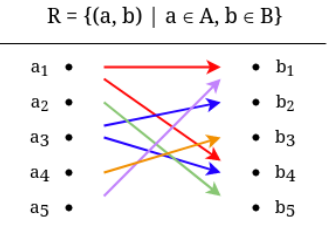
\includegraphics[width=.5\textwidth]{bigrafo.png}
                    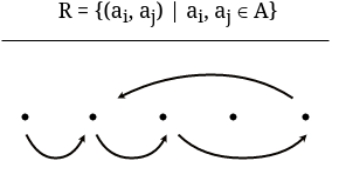
\includegraphics[width=.5\textwidth]{digrafo.png}
                    \caption{Dx: Bigrafo, Sx: Digrafo}
                \end{figure}
            \end{center}
        \subsubsubsection{Matrice binaria}
            Definiamo una matrice $M_R$ dove 
            $$M_{i,j} = \begin{cases}
                1 & \left(a_i, b_j\right) \in R\left(A, B\right) \\
                0 & \left(a_i, b_j\right) \notin R\left(A, B\right) \\
            \end{cases}$$
    \subsection{Relazione inversa}
        Data una relazione, \textbf{esiste sempre} l'inversa 
        $$R^{-1}=\{\left(b, a\right) \forall \left(a, b\right) \in R\}$$ 
        Quando $R^{-1} = R$ si parla di \textbf{relazione simmetrica}. 
        $$R\left(A, B\right) \textbf{ simmetrica } \Longleftrightarrow \left(a, b\right) = \left(b, a\right)$$
        \subsubsection{Corrispondenza con la trasposizione}
            Questa operazione corrisponde con la trasposizione della matrice $M_R$
            $$M_{R^{-1}} = {M_R}^T$$
            Possiamo inoltre facilmente dedurre che
            $$R \textrm{ simmetrica } \Longleftrightarrow M_{R^{-1}} = M_R$$
    \subsection{Composizione di relazioni}
        $$R \subseteq A \cdot B, S \subseteq B \cdot C \Longrightarrow R \circ S = 
        \left(a, c\right) \Longleftrightarrow \exists\left(a, b\right) \wedge \exists \left(b, c\right)$$
        Nei casi di $R \circ R$ parliamo di \textbf{iterazione}
        \subsubsection{Composizione di relazioni come prodotto fra matrici}
            $$M_{R,S} = M_R \cdot M_S$$
            Dove si usano la somma ed il prodotto booleano
        \subsubsection{Associatività}
            $$ R \circ \left(S \circ D\right) = \left(R \circ S\right) \circ D$$
            In quanto la moltiplicazione fra matrici è associativa, possiamo dedurre
            che lo è anche la composizione di relazioni in quanto operazioni equivalenti
        \subsubsection{Commutatività}
            $$ R \circ S \circ D \neq R \circ D \circ S $$
            Come prima, possiamo dedurlo dal fatto che il prodotto fra matrici non è
            commutativo
    \subsection{Relazioni transitive}
        $$R \subseteq A \cdot A \textrm{ transitiva } \Longleftrightarrow$$
        $$\left(\forall a, b, c \in A, \, aRb \wedge bRc \Longrightarrow aRc\right)$$
        \subsubsection{Chiusura transitiva}
            E' detta \textbf{chiusura transitiva} di $R$ \textbf{la più piccola 
            relazione transitiva} $R^T$ tale che:
            $$R \subseteq R^T \wedge R^T \textrm{ transitiva } \wedge R \subseteq S, \left(\textrm{S transitiva} \Longrightarrow R^T \subseteq S\right)$$
        \subsubsection{Cammino}
            $$R \subseteq A \cdot A, \exists x_0, x_1, ... \textrm{ t.c. } aRx_0Rx_1R...Rb$$
            $$\Longleftrightarrow \exists \textrm{ cammino } a \rightarrow b \textrm{ di lunghezza } l \geq 1$$
    \subsection{Relazione di equivalenza}
        \begin{itemize}
            \item Riflessiva: $\forall a \in A \, \exists aRa$
            \item Simmetrica: $\forall a,b \in A, \, aRb \Longrightarrow bRa$
            \item Transitiva: $\forall a,b,c \in A, \, aRb \wedge bRc \Longrightarrow aRc$
        \end{itemize} 
        \subsubsection{Classi di equivalenza}
            Preso $a \in A$, possiamo definire l'insieme 
                $$\left[a\right]_R = \{b \in A \mid aRb\}$$. 
            Questo insieme è detto \textbf{classe di equivalenza}
            Possiamo inoltre dire che:
            \begin{itemize}
                \item per la riflessività, $\forall a \in A \left[a\right]_R \neq \emptyset$
                \item per la simmetria e la transitività, 
                    $\forall a, b \in A \left[a\right]_R \cap \left[b\right]_R = \emptyset \vee \left[a\right]_R = \left[b\right]_R$
            \end{itemize}
        \subsubsection{Partizioni}
            Una partizione di un insieme $A$ è la famiglia $\{C_i \mid i \in I\}$ tali che
            \begin{itemize}
                \item $C_i \subseteq A$
                \item $C_i \neq \emptyset$
                \item $\forall a \in A \exists i \in I$ t.c. $a \in C_i$
                \item $\forall i, j \in I, i \neq j \Longrightarrow C_i \cap C_j = \emptyset$
                \item $\bigcup_{i \in I} C_i = A$
            \end{itemize}
            Possiamo quindi dire che
            $$\{C_i \mid i \in I\} \textrm{ partizione } A, R\left(A\right), 
                \left(aRb \Longleftrightarrow \exists i \in I \textrm{ t.c. } a, b \in C_i\right)
                \Longrightarrow R\left(A\right) \textrm{ relazione di equivalenza}
            $$
    \subsection{Relazioni d'ordine}
        Relazione binaria che gode di alcune proprietà della relazione $\leq\left(\mathbf{N}\right)$
        \subsubsection{Relazione d'ordine totale}
            \begin{itemize}
                \item Riflessiva: $\forall a \in A \, \exists aRa$
                \item Anti-simmetrica: $\forall a, b \in A, \, aRb \wedge bRa \Longrightarrow a = b$
                \item Transitiva: $\forall a,b,c \in A, \, aRb \wedge bRc \Longrightarrow aRc$
                \item Totale: $\forall a, b \in A, a \leq b \vee b \leq a$. Se questa proprietà non sussiste si parla di \textbf{ordine parziale}
            \end{itemize}
        $\emptyset$ e una qualunque $R\left(\emptyset\right)$ sono relazioni d'ordine.
        \subsubsection{Cicli}
           $$\forall R\left(A\right) \textrm{ ordine } \Longrightarrow \textrm{ lunghezza massimo ciclo } = 1$$
           \subsubsubsection{Dimostrazione}
                Ipotizziamo per assurdo che esista un ciclo di lunghezza $ > 1$, ovvero tale che 
                $$a_1Ra_2R...Ra_1, \textrm{ t.c. } \forall i, j \, i \neq j \Longrightarrow a_i \neq a_j$$
                Per transitività ripetuta abbiamo che $a_1Ra_i$, ma anche che $a_iRa_1,  \forall i \neq 1$. \\
                Per antisimmetria ciò implica che $a_i = a_1$, ovvero che tutti gli elementi del ciclo sono 
                lo stesso elemento. Ne consegue che il ciclo si può ridurre a $a_1Ra_1$, di lunghezza $1$.
        \subsubsection{Minimo e massimo di un ordine}
            $$a \in A \textrm{ t.c. } \forall b \in A \exists aRb / bRa \Longrightarrow a \textrm{ è minimo/massimo di } R\left(A\right)$$
            Non è garantita l'esistenza di questi elementi.
        \subsubsection{Minimali e massimale di un ordine}
            E' detto \textbf{minimale} $a \in R\left(A\right) \textrm{ t.c. } \forall b \in A, b \neq a, \, \nexists bRa$. \\
            Analogamente, è detto \textbf{massimale} $a \in R\left(A\right) \textrm{ t.c. } \forall b \in A, b \neq a, \, \nexists aRb$ \\
            Inoltre, $\forall R\left(A\right), A \textrm{ finito } \exists a \in A \textrm{ minimale } \wedge \exists b \in A \textrm{ massimale }$
            \subsubsubsection{Dimostrazione}
                Prendiamo il percorso $P$ più lungo $a_1Ra_2R...Ra_n$, dove $a_1$ minimale. \\ 
                Se $\exists a \in A, a \notin P$, non può valere $aRa_1$, in quanto esisterebbe 
                il percorso $aRa_1Ra_2R...Ra_n$, di lunghezza maggiore di $P$, impossibile per ipotesi. \\  
                Se invece $\exists a \in A, a \in P$ ne consegue che esiste un ciclo in $P$, impossibile 
                in quanto siamo in un ordine parziale. \\
                Ne segue che $a_1$ è il minimale di $R\left(A\right)$ 
        \subsubsection{Immersioni tra ordini}
            \textbf{Tutti gli ordini sono inclusioni insiemistiche}, ovvero:
            $$\begin{array}{c}
                \leq\left(X\right)\textrm{ ordine parziale }, \leq^{*}\left(X^{*}\right)\textrm{ ordine parziale } \\
                \Longrightarrow \exists f: X \rightarrow X^{*} \textrm{ iniettiva t.c. } \left(x \leq y 
                \Longleftrightarrow f\left(x\right) \leq^{*} f\left(y\right)\right)
            \end{array}$$
        \subsubsection{Immersione nell'insieme potenza}
            $$\exists \leq\left(X\right) \Longrightarrow \exists \textrm{ immersione } \subseteq\left(\mathcal{P}\left(X\right)\right)$$
            \subsubsubsection{Dimostrazione}
                Definiamo 
                $$f: X \rightarrow \mathcal{P}\left(X\right), \, f\left(x\right) = \{z \in X \mid z \leq x\}$$
                Verifichiamo l'iniettività per assurdo:
                $$\begin{array}{c}
                    \forall x, y \in X, y \neq x, f\left(x\right) = f\left(y\right), x \leq x, y \leq y \\
                    \Longrightarrow x \in f\left(x\right) \wedge y \in f\left(y\right) 
                    \Longrightarrow x \in f\left(y\right) \wedge y \in f\left(x\right) \\
                    \Longrightarrow x \leq y \wedge y \leq x \Longrightarrow y = x \textrm{ per anti-simmetria } \\
                    \Longrightarrow \textrm{ contraddizione }
                \end{array}$$
                Verifichiamo che $x \leq y \Longrightarrow f\left(x\right) \subseteq f\left(y\right)$:
                $$\begin{array}{c}
                    x = y \Longrightarrow f\left(x\right) = f\left(y\right) \Longrightarrow f\left(x\right) \subseteq f\left(y\right) \\
                    x < y \Longrightarrow x \in f\left(y\right), y \notin f\left(x\right)\\
                    \textrm{Inoltre, per transitività } \forall z \in f\left(x\right), z \leq x < y \Longrightarrow z < y \Longrightarrow z \in f\left(y\right) \\
                    \Longrightarrow \forall z \in f\left(x\right), z \in f\left(y\right) \wedge x \in f\left(y\right) \wedge y \notin f\left(x\right) \\
                    \Longrightarrow f\left(x\right) \subset f\left(y\right)
                \end{array}$$
                Verifichiamo anche l'implicazione opposta:
                $$x \in f\left(x\right), f\left(x\right) \subseteq f\left(y\right) \Longrightarrow x \in f\left(y\right) \Longrightarrow x \leq y$$
        \subsubsection{Estensioni totali di ordini parziali}
            $$\begin{array}{c}
                A = \{a_1, ..., a_n\}, R\left(A\right) \textrm{ ordine parziale } \Longrightarrow \\ 
                \exists R^{*}\left(A\right) \textrm{ ordine totale t.c. } R \subseteq R^* \\
                \Downarrow \\
                \forall a,b \in A, \, R\left(A\right) \textrm{ ordine parziale}, \nexists aRb \\
                \Longrightarrow \exists R^{'}\left(A\right) \supseteq R \textrm{ t.c. } \exists aR^{'}b 
            \end{array}$$ 
            \subsubsubsection{Dimostrazione per casi}
                $$\begin{array}{l}
                    \left(a, b\right) \in A \times A, \, X = \{x \in A \mid  xRa\} (x \leq a), \, Y = \{y \in A \mid bRx\} (x \geq b) \\
                    R^{'} = R \cup \left(X \times Y\right) \\
                    \nexists aRb \Longrightarrow \nexists x \in X \textrm{ t.c. } xRa \wedge bRx \Longrightarrow X \cap Y = \emptyset \\ \\
                    R \textrm{ riflessiva } \Longrightarrow R^{'} \textrm{ riflessiva } \\ \\
                    \textrm{Dimostriamo l'antisimmetria:} \\
                    \textrm{ Ipotizziamo } \forall x \in X, y \in Y \, \exists xR^{'}y \wedge \exists yR^{'}x \\
                    \Longrightarrow \left(xRy \vee \left(x, y\right) \in X \times Y\right) \wedge \left(yRx \vee \left(y, x\right) \in X \times Y\right) \\
                    \textrm{Ne consegue per casi:} \\
                    \begin{array}{l}
                        \left(x, y\right), \left(y, x\right) \Longrightarrow x \in X \cap Y \Longrightarrow \textrm{ impossibile } \\
                        \left(x, y\right), yRx \Longrightarrow xRa \Longrightarrow yRa \Longrightarrow y \in X \Longrightarrow y \in X \cap Y \Longrightarrow \textrm{ impossibile } \\
                        xRy, \left(y, x\right) \Longrightarrow bRx \Longrightarrow bRy \Longrightarrow y \in Y \Longrightarrow y \in X \cap Y \Longrightarrow \textrm{ impossibile } \\
                        xRy, yRx \Longrightarrow y = x \textrm { per antisimmetria }
                    \end{array} \\ \\
                    \textrm{Dimostriamo la transitività:} \\
                    \textrm{Ipotizziamo } \forall x, y, z \in X, \exists xR^{'}y \wedge \exists yR^{'}z \\
                    \Longrightarrow \left(xRy \vee \left(x, y\right) \in X \times Y\right) \wedge \left(yRz \vee \left(y, z\right) \in X \times Y\right) \\
                    \textrm{Ne consegue per casi:} \\
                    \begin{array}{l}
                        \left(x, y\right), \left(y, z\right) \Longrightarrow y \in X \wedge y \in Y \Longrightarrow y \in X \cap Y \Longleftrightarrow \textrm{ impossibile } \\
                        \left(x, y\right), yRz \Longrightarrow y \in Y \Longrightarrow bRy \Longrightarrow bRz \Longrightarrow z \in Y \Longrightarrow \left(x, z\right) \in X \times Y \Longrightarrow xR^{'}z \\
                        xRy, \left(y, z\right) \Longrightarrow y \in X \Longrightarrow \exists yRa \Longrightarrow xRa \Longrightarrow x \in X \Longrightarrow \left(x, z\right) \in X \times Y \Longrightarrow xR^{'}z \\
                        xRy, yRz \Longrightarrow xRz \Longrightarrow xR^{'}z
                    \end{array} 
                \end{array}$$
            \subsubsubsection{Dimostrazione per induzione}
                Consideriamo il problema nel caso $A = {a}$. Banale il fatto che $R$ parziale sia anche totale. \\
                Consideriamo ora un generico caso $A = {a_1, ..., a_n}$, dove abbiamo che $\exists a, b \in A$ t.c. $\nexists aRb \wedge \nexists bRa$. \\
                Sappiamo che $\exists a \in A$ minimale di $R$, ed escludiamolo da $A$.
                Nell'insieme $R\left(A \backslash \{a\}\right)$ abbiamo due casi:
                \begin{itemize}
                    \item $R\left(A \backslash \{a\}\right)$ totale: basta definire un nuovo ordine 
                        $$R_T = R\left(A \backslash \{a\}\right) \cup \{aRx \, \forall x \in R\left(A \backslash \{a\}\right)\}$$
                    \item $R\left(A \backslash \{a\}\right)$ parziale: ripetiamo lo stesso procedimento definito sopra 
                        finchè non trovaimo un $R\left(A \backslash \{a_{i_1}, ..., a_{i_n}\}\right)$ totale. \\
                        Sappiamo che suddetto caso esiste in quanto al limite si arriva a un caso dove $A = {a}$ che sappiamo essere totale.
                \end{itemize}
                Di conseguenza, per un qualunque $n$ sappiamo risolvere il caso $n-1$, ed avendo risolto $n-1$ sappiamo risolvere $n$
        \subsubsection{Sottosuccessioni}
            $$A, \exists S_A \Longleftrightarrow \exists j \in \left[i, i + \#S\right] \textrm{ t.c. } S_{j-i} = A_j \, \forall j$$
        \subsubsection{Sottosuccessioni monotone ed ordini totali}
            $$\forall n \geq 1, \, A = \{a_1, ..., a_{n^2+1}\} \textrm{ t.c. } R\left(A\right) \textrm{ ordine totale } 
                \Longrightarrow \exists S_A = \{a_i, ..., a_{i+n+1}\} \textrm{ monotona }$$
            \subsubsubsection{Dimostrazione}
                Ipotizziamo per assurdo che questa successione non esista. \\
                Consideriamo $f:\left[1, n^2 + 1\right] \left[1, n \right], 
                    f\left(x\right) = \ell_{\textrm{max}} S_A = \{a_i, ..., a_x\} \textrm{ monotona }$ \\
                Dato che $\frac{n^2+1}{n} = n$ resto $1 \Longrightarrow \exists \{i_1 < ... < i_{n+1}\} 
                    \textrm{ t.c. } f\left(i_1\right) = ... = f\left(i_{n+1}\right) = l$ \\
                Consideriamo quindi gli elementi $a_{i_1}, ..., a_{i_{n+1}}$ che sappiamo avere lo stesso $\ell_{\textrm{max}}$. \\
                Preso una qualunque coppia adiacente $a_{i_k}, a_{i_{k+1}}$, abbiamo due casi:
                \begin{itemize}
                    \item $a_{i_k} < a_{i_{k+1}} \Longrightarrow S_{A_{a_{i_k}}} = 
                        \{S_{A_{a_{i_k}}} < a_{i_{k+1}}\} \Longrightarrow k < \left(k + 1\right) \Longrightarrow \textrm{ impossibile }$
                    \item $a_{i_k} > a_{i_{k+1}}$
                \end{itemize}
                Ne consegue che 
                $$\forall k \in \left[1, n+1\right) \Longrightarrow a_{i_k} > a_{i_{k+1}} 
                    \Longrightarrow \exists S^* = \{x_{i_1} > ... > x_{i_{n+1}}\} \Longrightarrow \#S^* = n+1 \Longrightarrow \textrm{ contraddizione }$$
                Ergo l'ipotesi è falsa 
\newpage 
\section{Induzione}
    L'idea base del principio di induzione è dimostrare che 
    $$P\left(n\right) \forall n \in X \subseteq \mathbf{N}$$
    E' composta da due parti fondamentali: 
    \begin{itemize}
        \item \textbf{Caso base}: dimostrare che $\exists n_0 \in N \textrm{ t.c. } P\left(n\right)$ 
            Solitamente $n_0 = 0 \textrm{ o } 1$
        \item \textbf{Passo induttivo}: dimostrare che 
            $\forall n \in N, n \geq n_0, P\left(n\right) \Longrightarrow P\left(n+1\right)$. 
            L'ipotesi $P\left(n\right)$ è detta \textbf{ipotesi induttiva}
    \end{itemize}
    \subsection{Principio di Induzione: versione insiemistica}
        $$\begin{array}{l c}
            X \subseteq \mathbf{N} \\
            n_0 \in X & \\
            \forall n \in \mathbf{N}, n \geq n_0, n \in X \Longrightarrow n + 1 \in X & \\
            & \Longrightarrow \mathbf{N} - \{0, ..., n_0 - 1\} \subset X \Longrightarrow X = \mathbf{N} - \{0, ..., n_0 - 1\}
        \end{array}$$
    \subsection{Dimostrazione col Principio del Minimo Numero}
        Il principio del minimo numero ci dice che 
        $$\forall X \subseteq \mathbf{N}, X \neq \emptyset \Longrightarrow \exists m \in X$$
        Prendiamo le condizioni della versione insiemistica, ed ipotizziamo per assurdo che 
        l'induzione insiemistica non sia valida, ovvero che
        $$A = \mathbf{N} - \{0, ..., n_0 - 1\} - X, A \neq \emptyset$$
        Per il principio del minimo numero $\exists m \in A > n_0$ in quanto $n_0 \in X$, ovvero 
        $m - 1 \geq n_0$, e poichè è $m \in A \Longrightarrow m - 1 \in X$, ma poichè
        $\forall n \geq n_0, n \in X \Longrightarrow n + 1 \in X$ allora 
        $m - 1 \in X \Longrightarrow m \in X$, in contraddizione col fatto che $m \notin X$. \\
        Ne segue che l'induzione insiemistica è vera.
        \\
        La maggior parte delle dimostrazioni per PMN sono dimostrazioni per assurdo.
    \subsection{Mettere in evidenza il caso base}
        Il passaggio fondamentale nel processo di dimostrazione per induzione 
        è mettere in evidenza il caso $n$, ovvero mostrare il caso $n$ sia incluso nel caso 
        $n+1$. 
    \subsection{Principio di induzione forte}
        Il principio di induzione è una versione del principio di induzione dove 
        nel passo induttivo, oltre a considerare $P\left(n\right)$ vero, sfruttiamo il 
        fatto che $\forall x \in \left[n_0, n\right] P\left(n\right)$ vera 
\section{Logica proposizionale}
    Un linguaggio proposizionale è un insieme $L$ di simboli contenente:
    \begin{itemize}
        \item \textbf{Connettiviti logici}: $\implies, \iff, \neg, \lor, \land$
        \item \textbf{Parentesi}: $\left(\right)$
        \item \textbf{Variabili proposizionali}: Insieme $\textrm{VAR}_L$ di simboli diversi da connettivi e parentesi. 
            Data una proposizione $F$, sono anche dette \textbf{parti atomiche} di $F$
    \end{itemize}
    L'insieme delle \textbf{proposizioni} ($\textrm{PROP}_L$) di $L$ è il minimo insieme $X$ di stringhe
    finite di simboli in $L$ t.c.:
    \begin{itemize}
        \item $\textrm{VAR}_L \subset X$
        \item $A \in X \implies \neg A \in X$
        \item $A, B \in X \implies A \lor/\land/\implies/\iff B \in X$
    \end{itemize}
    \subsection{Connettivi logici nell'algebra booleana}
        \begin{itemize}
            \item $\neg A = \overline{A}$
            \item $A \land B = A \cdot B$
            \item $A \lor B = A \lor B$
            \item $A \implies B = \overline{A \cdot \overline{B}}$
            \item $A \iff B = AB + \overline{A}\overline{B}$
        \end{itemize}
        Valgono di conseguenza le leggi e i metodi di rappresentazione dell'algebra booleana.
    \subsection{Sottoformule}
        $$A, B \in \textrm{PROP}_L, B \textrm{sottostringa di } A \implies B \textrm{ sottoformula } A$$
    \subsection{Semantica della Logica proposizionale}
        \subsubsection{Assegnamento}
            $$\alpha: \textrm{VAR} \rightarrow \{0,1\}$$
            $0,1$ sono detti \textbf{valori di verità}.
            Il concetto è estensibilie alle proposizioni, dove $\alpha\left(F\right)$, detta anche 
            $F$ sotto $\alpha$, è l'insieme degli assegnamenti alle atomiche 
        \subsubsection{Soddisfacibile, Insoddisfacibile e Tautologica}
            $$\exists \alpha \in A \textrm{ t.c. } \alpha\left(F\right) = 1 \iff F \in \textrm{ SAT}$$
            $$\forall \alpha \in A, \alpha\left(F\right) = 1 \iff F \in \textrm{ TAUT}$$
            $$\neg A \in \textrm{ TAUT} \iff A \in \textrm{ UNSAT}$$
        \subsubsection{Conseguenza logica}
            $$\forall \alpha \in A, \left[1 = \alpha\left(F_1\right) = ... = \alpha\left(F_n\right) 
                \implies \alpha\left(F\right) = 1\right] \implies F_1, ..., F_n \models F$$
            $F$ è detta \textbf{conseguenza logica} di $F_1, ..., F_n$ \\
            Il contrario è 
            $$\exists \alpha \in A, \left[1 = \alpha\left(F_1\right) = ... = \alpha\left(F_n\right) 
                \wedge \alpha\left(F\right) = 0\right] \implies F_1, ..., F_n \not\models F$$
        \subsubsection{Conseguenza logica come espressione booleana}
            $$\forall \alpha \in A, \left[F_1 \cdot ... \cdot F_n \cdot F\right] = 1 
                \implies F_1, ..., F_n \models F_1$$
            $$\exists \alpha \in A, \left[F_1 \cdot ... \cdot F_n \cdot \neg F\right] = 1 
                \implies F_1, ..., F_n \not\models F_1$$
        \subsubsection{Conseguenza logica come UNSAT e TAUT}
            $$F_1, ..., F_n \models F 
                \iff \left[F_1 \wedge ... \wedge F_n \implies F\right] \in \textrm{ TAUT} 
                \iff \left[F_1 \wedge ... \wedge F_n \wedge F\right] \in \textrm{ UNSAT}
            $$
        \subsubsection{Forma Normale Congiunta}
            La \textbf{CNF}, sempre possibile, sarebbe un modo di scrivere la formula 
            $F$ nella forma 
            $$F = \bigwedge_{i=1}^n C_i = \bigwedge_{i=1}^n \bigvee_{j=1}^{m_i} l_{j_i}$$
            Facile notare come sia la POS \\
            La CNF è reinscrivibile in forma insiemistica come 
            $$\{\{l_{1_1}, ..., l_{1_m}\}, ..., \{l_{n_1}, l_{n_m}\}\}$$
        \subsubsection{Metodo di risoluzione}
            Il metodo di risoluzione è un modo per scoprire se $F$ è Insoddisfacibile o meno. \\
            Il metodo si basa sul fatto che, in una F in CNF:
            $$\exists C_1, C_2 \in F \textrm{ t.c. } \exists l_1 \in C_1, l_2 \in C_2 \textrm{ t.c. } l_1 = \neg l_2$$
            L'algoritmo è il seguente:
            $$l_1 \in C_1, \neg l_1 \in C_2 \Longrightarrow C_1, C_2 \models \textrm{RIS}\left(C_1, C_2\right) = C_1 \cup C_2 - \{l_1, \neg l_1\}$$
            E' possibile quindi sostituire $C_1 \land C_2$ con la loro risoluzione. \\
            Il processo finisce quando RIS$\left(C_1, C_2\right) = \{\} = \square$. \\
            Dimostriamo ora che $\square \in F \iff F \in$ UNSAT
            \subsubsubsection{Dimostrazione \textit{"da sinistra"}}
                Facile notare come RIS$\left(C_1, C_2\right)$ si ottiene solamente quando $C_1 = \{p\} \land C_2 = \{\neg p\}$, 
                ovvero $p \times \neg p$, che sappiamo essere un'espressione UNSAT
            \subsubsubsection{Dimostrazione \textit{"da destra"}}
                Dimostriamolo per induzione:
                \begin{itemize}
                    \item Caso base: $n = 0 \implies F = \{\square\} \vee F = \emptyset, 
                        F \in \textrm{ UNSAT} \implies F = \{\square\}$
                    \item Passo Induttivo: Abbiamo due casi anche qui: \\
                        Consideriamo i tre insiemi:
                        $$F_p = \{C \in F \mid p \in C\}, F_{\neg p} = \{C \in F \mid \neg p \in C\}, F^- = F - F_p - F_{\neg p}$$
                        $$\textrm{RIS}\left(F_p, F_{\neg p}\right) = \left(D = F_p - \{p\}\right) \cup \left(E = F_{\neg p} - \{\neg p\}\right)$$
                        $$R = D \cup E \cup F^- \textrm{ (questo processo è equivalente al metodo di risoluzione) } = F^- \times D \times E$$
                        Dimostriamo per assurdo che $R$ è UNSAT: \\
                        $\exists \alpha \textrm{ t.c. } \alpha\left(R\right) = 1 \implies \alpha\left(D \times E\right) = 1$.
                        Definiamo $\alpha_1 = \alpha, \alpha\left(p\right) = 1$ e $\alpha_0 = \alpha, \alpha\left(p\right) = 0$ \\
                        \begin{itemize}
                            \item $\alpha_1\left(F\right) = 0 \implies \forall C_p \in F_p: \alpha_1\left(C_p\right) = 1 \implies 
                                \exists C_{\neg p} \in F_{\neg p}: \alpha_1\left(C_{\neg p}\right) = 0$ \\
                                In quanto possiamo ignorare $\neg p$ in quanto $= 0$, ne consegue che 
                                $\alpha_1\left(C_{\neg p} - \{\neg p\}\right) = 0 \implies \alpha\left(C_{\neg p} - \{\neg p\}\right) = 0$ \\
                                Quest'ultima osservazione implica per costruzione $\alpha\left(E\right) = 0$
                            \item Analogamente per $\alpha_0$ e $C_p - \{p\}$. Concludiamo che $\alpha\left(D\right) = 0$
                        \end{itemize}
                        $\alpha\left(D \times E\right) = 1 \implies \alpha\left(D\right) = 1$, contraddizione e di conseguenza cade l'argomento. \\
                        Abbiamo quindi dimostrato che $R$ è UNSAT, e quindi che $\square \in \textrm{RIS}\left(R\right)$, 
                        ottenuta applicando il metodo di risoluzione. Q.E.D
                \end{itemize}
\end{document}
